
% xetex expected
\documentclass[xetex,professionalfont]{beamer}

% we want math
\usepackage{amsmath}

% fixes and extensions to amsmath
\usepackage{mathtools}

% additional math symbols
\usepackage{amssymb}

% good-looking fractions in text via \sfrac
\usepackage{xfrac}

% fix spaces after custom commands (see below for examples)
\usepackage{xspace}

% minted allows for fancy syntax highlighting (requires python with pygments)
% usage:
%   \begin{minted}{python}
%   codeb
%   \end{minted}
\usepackage{minted}

% better looking tables
% usage:
%   begin with a \toprule, write a single row of column headings,
%   then add \midrule and after the columns of data we finish with \bottomrule
% example:
%   \begin{tabular}{llr} \toprule
%   Animal & Description & Price \midrule
%   cat & foo & 10 \\
%   dog & bar & 20 \\ \bottomrule
%   \end{tabular}
% note that good tables generally neither have vertical rules nor double rules
\usepackage{booktabs}

% system font support (requires xetex or luatex)
\usepackage{fontspec}
\setmonofont[Scale=0.7]{Cousine} % part of ttf-chromeos fonts on Arch

% improve microtypography
\usepackage{microtype}

% multi-language quotes for babel
\usepackage{csquotes}

% easy way to include copyright information
\usepackage{copyrightbox}

% better bibliographies
\usepackage[backend=biber,style=authoryear]{biblatex}

% language support (english,ngerman)
\usepackage[english]{babel}

% -----------------------------------------------------------------------------

% specify PDF metadata
\hypersetup{pdftitle={CVSP VO - IP Recap},pdfsubject={},pdfauthor={Christopher Pramerdorfer}}

% copyright font style
\makeatletter\renewcommand{\CRB@setcopyrightfont}{\tiny\color{lightgray}}

% make emph bold
\DeclareTextFontCommand{\emph}{\bfseries}

% use proper fonts for math
% \usefonttheme[onlymath]{serif}

% use tuwcvl beamer theme
\usetheme{tuwcvl}

% add bib file
\addbibresource{literature.bib}

% -----------------------------------------------------------------------------

% common english abbreviations
\newcommand{\ie}{\mbox{i.e.}\xspace} % i.e.
\newcommand{\eg}{\mbox{e.g.}\xspace} % e.g.

% math - argmin and argmax
\DeclareMathOperator*{\argmin}{arg\,min}
\DeclareMathOperator*{\argmax}{arg\,max}

% shortcuts for number ranges
\newcommand{\NN}{\mathbb{N}}
\newcommand{\ZZ}{\mathbb{Z}}
\newcommand{\QQ}{\mathbb{Q}}
\newcommand{\RR}{\mathbb{R}}

% bold vectors
\renewcommand{\vec}[1]{\ensuremath{\mathbf{#1}}}

% vector shortcuts
\newcommand{\va}{\vec{a}}
\newcommand{\vb}{\vec{b}}
\newcommand{\vc}{\vec{c}}
\newcommand{\ve}{\vec{e}}
\newcommand{\vr}{\vec{r}}
\newcommand{\vs}{\vec{s}}
\newcommand{\vt}{\vec{t}}
\newcommand{\vu}{\vec{u}}
\newcommand{\vv}{\vec{v}}
\newcommand{\vw}{\vec{w}}
\newcommand{\vx}{\vec{x}}
\newcommand{\vy}{\vec{y}}
\newcommand{\vz}{\vec{z}}

% -----------------------------------------------------------------------------

\title{Computer Vision Systems Programming VO}
\subtitle{A Recap of Image Processing}
\author{Christopher Pramerdorfer}
\institute{Computer Vision Lab, Vienna University of Technology}

\begin{document}

% -----------------------------------------------------------------------------

\begin{frame}
\maketitle
\end{frame}

% -----------------------------------------------------------------------------

\begin{frame}
\frametitle{Topics}

A brief recap of Image Processing (IP)
\begin{itemize}
	\item Assuming you are already familiar with IP
	\item Focus on methods that are widely used in practice
\end{itemize}

\medskip
\begin{center}
	\copyrightbox[b]
	{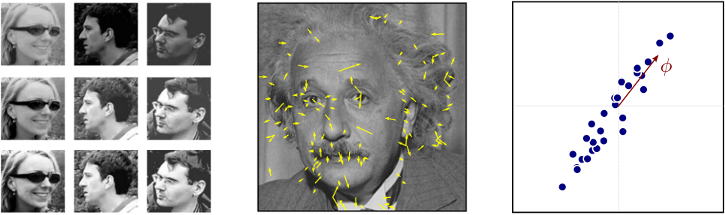
\includegraphics[width=8cm]{figures/intro-collage.png}}
	{\centering Images from \cite{prince12}}
\end{center}

\end{frame}

% -----------------------------------------------------------------------------

\begin{frame}
\frametitle{Relation of IP and CV}

IP encompasses operations that
\begin{itemize}
	\item Take images as input
	\item Produce images or representations (\eg descriptors)
\end{itemize}

\medskip
We regard IP as preprocessing for CV
\begin{itemize}
	\item IP has great influence on CV performance
\end{itemize}

\end{frame}

% -----------------------------------------------------------------------------

\begin{frame}
\frametitle{Contrast Normalization}

Reduce variation due to contrast and intensity changes

\bigskip
We cover two techniques
\begin{itemize}
	\item Whitening
	\item Histogram equalization
\end{itemize}

\medskip
\begin{center}
	\copyrightbox[b]
	{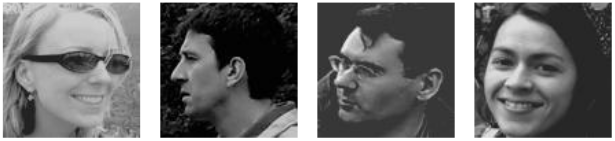
\includegraphics[width=8cm]{figures/contrast-original.png}}
	{\centering Images from \cite{prince12}}
\end{center}

\end{frame}

% -----------------------------------------------------------------------------

\begin{frame}
\frametitle{Contrast Normalization}
\framesubtitle{Whitening}

Transform pixel values so that
\begin{itemize}
	\item Their mean is zero
	\item Their variance is one % i.e. the resulting values are floats. if required, the result can be mapped to [0, 255] again by mapping -1 to 0 and 1 to 255, for example
\end{itemize}

\medskip
\begin{center}
	\copyrightbox[b]
	{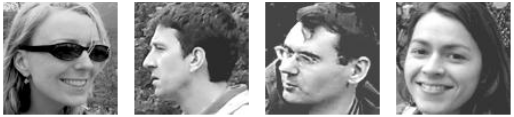
\includegraphics[width=8cm]{figures/contrast-whitening.png}}
	{\centering Images from \cite{prince12}}
\end{center}

\end{frame}

% -----------------------------------------------------------------------------

\begin{frame}[fragile]
\frametitle{Contrast Normalization}
\framesubtitle{Whitening -- Matlab Implementation}

\begin{minted}{matlab}
img = single(rgb2gray(imread('image.png'))); % load
m = mean(img(:)); % compute mean
s = std(img(:)); % compute standard deviation
whitened = (img - m) / s; % normalize
\end{minted}{matlab}

\end{frame}

% -----------------------------------------------------------------------------

\begin{frame}
\frametitle{Contrast Normalization}
\framesubtitle{Histogram equalization}

Transform pixel values so that distribution is \enquote{flat} % not exactly flat because input is descrete (see example images on Wikipedia)
\begin{itemize}
	\item Cumulative histogram linear over value range % like 0 ... 255 in 8-bit case
\end{itemize}

\medskip
\begin{center}
	\copyrightbox[b]
	{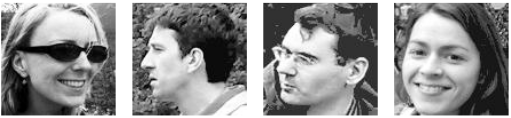
\includegraphics[width=8cm]{figures/contrast-histeq.png}}
	{\centering Images from \cite{prince12}}
\end{center}

\end{frame}

% -----------------------------------------------------------------------------

\begin{frame}[fragile]
\frametitle{Contrast Normalization}
\framesubtitle{Histogram Equalization -- C++ Implementation}

\begin{minted}{cpp}
// cv = OpenCV namespace
cv::Mat img, equalized; // storage
img = cv::imread("image.png", CV_LOAD_IMAGE_GRAYSCALE); // load
cv::equalizeHist(img, equalized); // normalize
\end{minted}{cpp}

\end{frame}

% -----------------------------------------------------------------------------

\begin{frame}
\frametitle{Noise Reduction and Change Detection}

Reduce image noise\\\medskip
Locate intensity changes

\bigskip
Accomplished via \emph{linear filtering} (but there are other means)
\begin{itemize}
	\item Pixel values linear combination of neighbor values
	\item Computed via convolution (or correlation)
\end{itemize}

\[
f'(x,y) = \sum_{i,j}f(x-i,y-j)h(i,j) % with convolution the kernel is flipped (x-i,y-j), with correlation this is not the case (x+i,y+j) ... most IP kernels are symmetric so the result is the same
\]

\end{frame}

% -----------------------------------------------------------------------------

\begin{frame}
\frametitle{Noise Reduction and Change Detection}
\framesubtitle{Noise Reduction via Blurring}

Use a 2D Gaussian as kernel $h$:
\[
h(i,j)=\frac{1}{2\pi\sigma^2}\exp\left(-\frac{i^2+j^2}{2\sigma^2}\right)
\]

\begin{center}
	\copyrightbox[b]
	{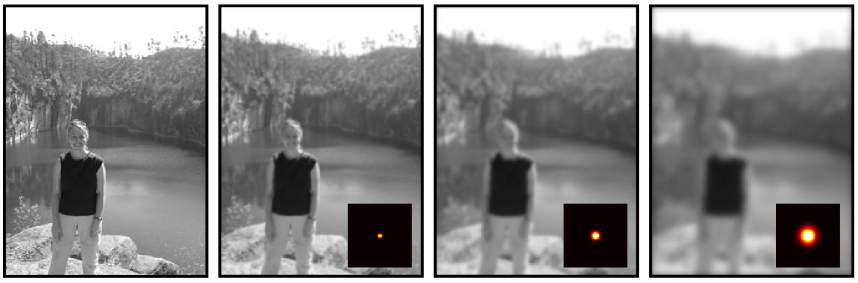
\includegraphics[width=8cm]{figures/linear-blur.png}}
	{\centering Images from \cite{prince12}}
\end{center}

\end{frame}

% -----------------------------------------------------------------------------

\begin{frame}[fragile]
\frametitle{Noise Reduction and Change Detection}
\framesubtitle{Noise Reduction via Blurring -- Matlab Implementation}

\begin{minted}{matlab}
img = rgb2gray(imread('image.png')); % load
h = fspecial('gaussian', [3 3], 0.5); % create Gaussian kernel
filtered = imfilter(img, h); % filter
\end{minted}{matlab}

\end{frame}

% -----------------------------------------------------------------------------

\begin{frame}
\frametitle{Noise Reduction and Change Detection}
\framesubtitle{Change Detection via LoG Filtering}

Use a Laplacian of Gaussian (LoG) filter as kernel $h$ % for 3x3 this is just [0 -1 0 ; -1 4 -1 ; 0 -1 0]
\begin{itemize}
	\item Gaussian for noise reduction
	\item Laplacian approximates $\nabla^2=f_{xx}+f_{yy}$ % sum of second pure derivatives of image
\end{itemize}

\bigskip
LoG filters respond to intensity changes % strong response near corners, zero crossing on corners
\begin{itemize}
	\item Regardless of direction
	\item At a frequency defined by $\sigma$ of Gaussian
\end{itemize}

\bigskip
Substrate for SIFT interest points % SIFT actually used differences of Gaussians to approximate LoG, which is faster

\end{frame}

% -----------------------------------------------------------------------------

\begin{frame}
\frametitle{Noise Reduction and Change Detection}
\framesubtitle{Change Detection via LoG Filtering}

\begin{center}
	\copyrightbox[b]
	{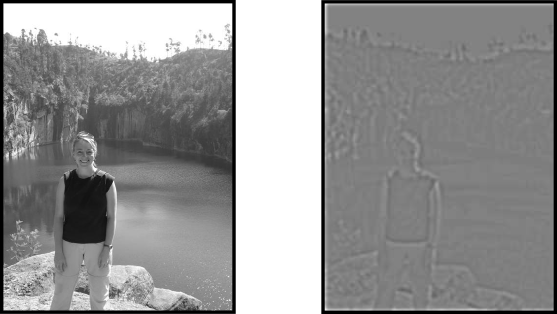
\includegraphics[width=7cm]{figures/linear-log.png}}
	{\centering Images from \cite{prince12}}
\end{center}

\end{frame}

% -----------------------------------------------------------------------------

\begin{frame}
\frametitle{Noise Reduction and Change Detection}
\framesubtitle{Change Detection via Gabor Filtering}

Use a Gabor filter as kernel $h$, which consists of
\begin{itemize}
	\item A Gaussian for noise reduction
	\item A Sinusoid for change detection 
\end{itemize}

\bigskip
Gabor filters respond to intensity changes at a
\begin{itemize}
	\item Phase and orientation defined by the Sinusoid % phase, orientation, wavelength, but can be made independent of phase by summing squared responses of two filters with pi/2 phase shift
	\item Frequency defined by the Gaussian and Sinusoid
\end{itemize}

\bigskip
Substrate for object recognition and scene understanding

\end{frame}

% -----------------------------------------------------------------------------

\begin{frame}
\frametitle{Noise Reduction and Change Detection}
\framesubtitle{Change Detection via Gabor Filtering}

\begin{center}
	\copyrightbox[b]
	{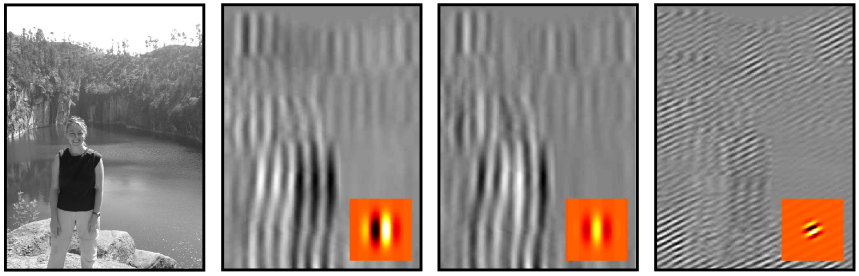
\includegraphics[width=10cm]{figures/linear-gabor.jpg}}
	{\centering Images from \cite{prince12}}
\end{center}

\end{frame}

% -----------------------------------------------------------------------------

\begin{frame}[fragile]
\frametitle{Noise Reduction and Change Detection}
\framesubtitle{Change Detection via Gabor Filtering -- C++ Implementation}

% OpenCV does not provide LoG filters, so we can either create them by
% convolving a Gaussian and a Laplacian or we can apply both filters consecutively
% this is possible because convolution is associative

\begin{minted}{cpp}
cv::Mat img, gabor; // storage
img = cv::imread("image.png", CV_LOAD_IMAGE_GRAYSCALE); // load
h = cv::getGaborKernel(...); // create Gabor kernel
cv::filter2D(img, gabor, CV_32F, h); // filter

\end{minted}{cpp}

\end{frame}

% -----------------------------------------------------------------------------

\begin{frame}
\frametitle{Interest Point Detection}

Interest points are image locations that
\begin{itemize}
	\item Can be detected reliably in multiple images of the same object
	\item Which means they are \emph{invariant} to image transformations
\end{itemize} % this is not very precise, see Tuytelaars08 for more information

\bigskip
This excludes everything but \enquote{corners} (aperture problem) % corners = points whose intensity varies in more than one direction

\begin{center}
	\copyrightbox[b]
	{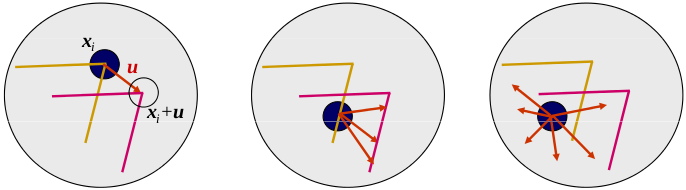
\includegraphics[width=8cm]{figures/aperture-problem.png}}
	{\centering Images from \cite{szeliski2010}}
\end{center}

\end{frame}

% -----------------------------------------------------------------------------

\begin{frame}
\frametitle{Interest Point Detection}
\framesubtitle{Harris Corner Detector}

Corners characterized by intensity change in multiple directions

\bigskip
Harris corner detector exploits this by
\begin{itemize}
	\item Checking gradient distribution in local neighborhood
	\item Corner: gradient distribution has two large eigenvalues
\end{itemize}

\begin{center}
	\copyrightbox[b]
	{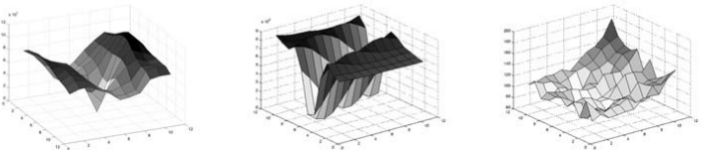
\includegraphics[width=8cm]{figures/cornerness.png}}
	{\centering Images from \cite{szeliski2010}}
\end{center}

\end{frame}

% -----------------------------------------------------------------------------

\begin{frame}
\frametitle{Interest Point Detection}
\framesubtitle{Harris Corner Detector}

Harris interest points
\begin{itemize}
	\item Are invariant to translation and rotation
	\item Stable under varying lighting conditions % because they are based on derivatives
\end{itemize} % they are also among the most repeatable and most informative, see Tuytelaars08

\medskip
\begin{center}
	\copyrightbox[b]
	{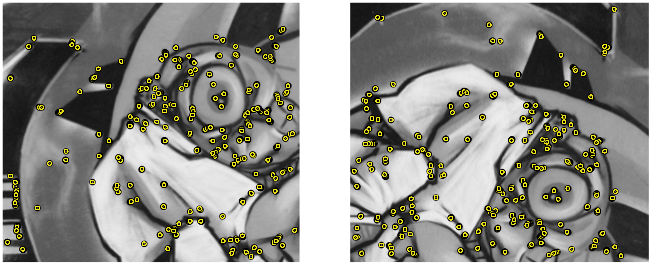
\includegraphics[width=8cm]{figures/ip-harris.png}}
	{\centering Images from \cite{tuytelaars2008}}
\end{center}

\end{frame}

% -----------------------------------------------------------------------------

\begin{frame}[fragile]
\frametitle{Interest Point Detection}
\framesubtitle{Harris Corner Detector -- Matlab Implementation}

\begin{minted}{matlab}
img = rgb2gray(imread('image.png')); % load
corners = corner(img, 'Harris', maxNum); % detect corners
\end{minted}{matlab}

\end{frame}

% -----------------------------------------------------------------------------

\begin{frame}
\frametitle{Bibliography}

\printbibliography

\end{frame}

\end{document}